\chapter{Análisis}

\section{Product Backlog}
En esta sección, en la Tabla~\ref{tab:huprioridad}, se ordenan las historias de usuario por prioridad, teniendo en cuenta las dependencias existentes entre las mismas. Se ha optado por una ordenación numérica, de mayor a menor prioridad, con el objetivo de evitar cuellos de botella.

\rowcolors{2}{grisfila}{white}
\begin{longtable}{>{\centering\arraybackslash}m{1.5cm} m{8cm} >{\centering\arraybackslash}m{2cm}}

\caption{Orden del product backlog}
\label{tab:huprioridad} \\    

\toprule
\rowcolor{grisfila}
\textbf{Código} & \multicolumn{1}{c}{\textbf{Título}} & \textbf{Prioridad}\\
\midrule
HU1 & Como cliente quiero poder crearme un perfil para poder usar la aplicación & 1 \\
HU22 & Como administrador quiero poder crear otro administrador para que me ayude en las tareas de gestión & 2 \\
HU4 & Como usuario quiero poder iniciar sesión en la aplicación para acceder a sus funcionalidades & 3\\
HU5 & Como usuario quiero poder cerrar sesión en la aplicación para que nadie más pueda acceder a mi cuenta & 4\\
HU2 & Como usuario quiero poder editar mi perfil para modificar mis datos & 5\\
HU3 & Como cliente quiero poder eliminar mi perfil para eliminar mis datos de la aplicación & 6\\
HU23 & Como administrador quiero poder eliminar a otro administrador para revocar sus permisos de administración & 7\\
HU6 & Como cliente quiero poder crear un grupo para tomar decisiones con mis amigos & 8\\
HU8 & Como cliente quiero poder añadir miembros a un grupo para añadirlos en la toma de decisiones & 9\\
HU7 & Como cliente quiero poder abandonar un grupo para dejar de formar parte de él & 10\\
HU9 & Como cliente quiero poder eliminar miembros de un grupo para que dejen de formar parte del grupo & 11\\
HU21 & Como cliente quiero poder subir imágenes a la aplicación para usarlas en las opciones o como foto de perfil o grupo & 12\\
HU24 & Como administrador quiero poder modificar los datos de un usuario para solucionar problemas de gestión & 13\\
HU25 & Como administrador quiero poder modificar datos de un grupo para solucionar problemas de gestión & 14\\
HU27 & Como administrador quiero poder eliminar un usuario para solucionar problemas de gestión & 15\\
HU10 & Como cliente quiero poder iniciar una votación para tomar una decisión & 16\\
HU17 & Como cliente quiero poder elegir el tipo de votación para adaptarlo a mis necesidades & 17\\
HU11 & Como cliente quiero asignarle un tiempo máximo a una votación para recibir los resultados en un tiempo limitado & 18\\
HU12 & Como cliente quiero poder editar una votación que haya creado para editar la decisión & 19\\
HU13 & Como cliente quiero poder eliminar una votación para cancelar una decisión & 20\\
HU16 & Como cliente quiero poder añadir opciones a una votación para poder votarlas posteriormente & 21\\
HU14 & Como cliente quiero poder ver las votaciones activas en los grupos a los que pertenezco para poder votar en ellas & 22\\
HU15 & Como cliente quiero poder votar en las votaciones para tener derecho de elección & 23\\
HU28 & Como administrador quiero poder eliminar un grupo para solucionar problemas de gestión & 24\\
HU26 & Como administrador quiero poder modificar datos de una votación para solucionar problemas de gestión & 25\\
HU19 & Como cliente quiero ver la opción ganadora en una votación para conocer la decisión final & 26\\ 
HU20 & Como cliente quiero poder seleccionar decisiones predeterminadas para facilitar mi toma de decisiones & 27\\
HU18 & Como cliente quiero ver las decisiones pasadas para recordar las elecciones tomadas & 28\\
HU29 & Como administrador quiero poder eliminar una votación para solucionar problemas de gestión & 29\\

\end{longtable}


\section{Tarjetas de usuario}
A continuación, exponemos las distintas historias de usuario desglosadas en tarjetas de usuario.

%1
\begin{hu_card}{1}{Como cliente quiero poder crearme un perfil para poder usar la aplicación}
    \begin{tabularx}{\linewidth}{l X}
        \textbf{Prioridad:}   & 1 \\
        \textbf{Estimación:}  & 2 PH \\
        \textbf{RF Relacionados:} & REQ1 \\
        \textbf{Categoría:} & Gestión de cuenta \\
    \end{tabularx}

    \vspace{2mm}
    \hrule
    \vspace{2mm}

    \textbf{Descripción Detallada:} \\
    Permitirá crear un nuevo cliente en el sistema.

    \vspace{2mm}
    \textbf{Tareas:}
    \begin{itemize}[noitemsep, topsep=0pt]
        \item Guardar el nuevo usuario en el sistema.
        \item Validar los datos introducidos.
        \item Crear una interfaz de creación de usuario.
    \end{itemize}

    \vspace{2mm}
    \textbf{Pruebas de Validación:}
    \begin{enumerate}[noitemsep, topsep=0pt]
        \item El sistema no permitirá el registro de usuarios con un correo electrónico ya existente en la base de datos.
        \item El sistema validará que el correo electrónico introducido cumple el formato estándar. Siendo el formato estándar:
            \begin{itemize}
                \item Contiene un único arroba (@), el cual no podrá ser ni el primer ni el último caracter.
                \item Presenta un punto después del arroba (@).
                \item Entre el arroba (@) y el punto debe aparecer al menos un caracter.
                \item Después del último punto hay al menos dos caracteres.
                \item No contiene espacios en blanco.
            \end{itemize}
        \item El nombre de usuario no podrá estar repetido en el sistema y no podrá contener el caracter arroba (@).
        \item La contraseña introducida deberá contener al menos 8 caracteres, una letra mayúscula, un número y un carácter especial.
        \item El campo de contraseña debe poder estar oculto mientras el usuario escribe.
        \item El campo de contraseña y confirmación deben coincidir.
        \item El usuario deberá confirmar su cuenta mediante el correo electrónico.
        \item La contraseña debe guardarse en el sistema encriptada.
        \item El sistema comprobará que la contraseña introducida no pertenece a una lista negra.
        \item El sistema mostrará mensajes de error claros indicando el motivo por el cual no puede crearse el usuario.
        \item Todos los campos obligatorios deberán estar rellenos.
    \end{enumerate}
\end{hu_card}

%2
\begin{hu_card}{2}{Como usuario quiero poder editar mi perfil para modificar mis datos}
    \begin{tabularx}{\linewidth}{l X}
        \textbf{Prioridad:}   & 5 \\
        \textbf{Estimación:}  & 1 PH  \\
        \textbf{RF Relacionados:} & REQ2\\
        \textbf{Categoría:} & Gestión de cuenta \\
    \end{tabularx}

    \vspace{2mm}
    \hrule
    \vspace{2mm}

    \textbf{Descripción Detallada:} \\
    El cliente podrá modificar todos sus datos personales introducidos en el sistema, teniendo estos nuevos datos que cumplir las mismas restricciones que se comprueban en el registro.

    \vspace{2mm}
    \textbf{Tareas:}
    \begin{itemize}[noitemsep, topsep=0pt]
        \item Crear la interfaz de modificación.
        \item Validar los datos introducidos.
        \item Modificar los datos guardados en la base de datos.
    \end{itemize}

    \vspace{2mm}
    \textbf{Pruebas de Validación:}
    \begin{enumerate}[noitemsep, topsep=0pt]
        \item El sistema no permitirá cambiar el correo electrónico a uno ya existente en la base de datos.
        \item El sistema validará que el correo electrónico introducido cumple el formato estándar. Siendo el formato estándar: 
            \begin{itemize}
                \item Contiene un único arroba (@), el cual no podrá ser ni el primer ni el último caracter.
                \item Presenta un punto después del arroba (@).
                \item Entre el arroba (@) y el punto debe aparecer al menos un caracter.
                \item Después del último punto hay al menos dos caracteres.
                \item No contiene espacios en blanco.
            \end{itemize}
        \item El nombre de usuario no podrá estar repetido en el sistema y no podrá contener el caracter arroba (@).
        \item La contraseña introducida deberá contener al menos 8 caracteres, una letra mayúscula, un número y un carácter especial.
        \item El campo de contraseña debe poder estar oculto mientras el usuario escribe.
        \item El campo de contraseña y confirmación deben coincidir.
        \item El usuario deberá confirmar su nuevo correo electrónico.
        \item La contraseña debe guardarse en el sistema encriptada.
        \item El sistema comprobará que la contraseña introducida no pertenece a una lista negra.
        \item El sistema mostrará mensajes de error claros indicando que campos del usuario no han podido modificarse.
    \end{enumerate}
\end{hu_card}

%3
\begin{hu_card}{3}{Como cliente quiero poder eliminar mi perfil para eliminar mis datos de la aplicación}
    \begin{tabularx}{\linewidth}{l X}
        \textbf{Prioridad:}   & 6 \\
        \textbf{Estimación:}  & 1 PH \\
        \textbf{RF Relacionados:} & REQ3 \\
        \textbf{Categoría:} & Gestión de cuenta \\
    \end{tabularx}

    \vspace{2mm}
    \hrule
    \vspace{2mm}

    \textbf{Descripción Detallada:} \\
    Permitirá que un usuario borre su cuenta del sistema.

    \vspace{2mm}
    \textbf{Tareas:}
    \begin{itemize}[noitemsep, topsep=0pt]
        \item Crear la interfaz con botón de eliminación.
        \item Eliminar la cuenta y los datos del usuario de los grupos y votaciones de la base de datos.
    \end{itemize}

    \vspace{2mm}
    \textbf{Pruebas de Validación:}
    \begin{enumerate}[noitemsep, topsep=0pt]
        \item La cuenta se borra del sistema.
        \item Se elimina la cuenta de los grupos a los que pertenezca y las votaciones en las que haya participado. 
        \item Al borrar la cuenta se redirige a la pantalla de inicio de sesión.
    \end{enumerate}
\end{hu_card}

%4
\begin{hu_card}{4}{Como usuario quiero poder iniciar sesión en la aplicación para acceder a sus funcionalidades}
    \begin{tabularx}{\linewidth}{l X}
        \textbf{Prioridad:}   & 3 \\
        \textbf{Estimación:}  & 1 PH \\
        \textbf{RF Relacionados:} & REQ23 \\
        \textbf{Categoría:} & Gestión de cuenta \\
    \end{tabularx}

    \vspace{2mm}
    \hrule
    \vspace{2mm}

    \textbf{Descripción Detallada:} \\
    Permitirá a un usuario entrar en la aplicación con los datos de la cuenta que tiene asociada en el sistema.

    \vspace{2mm}
    \textbf{Tareas:}
    \begin{itemize}[noitemsep, topsep=0pt]
        \item Crear la interfaz de inicio de sesión.
        \item Validar credenciales con la base de datos.
    \end{itemize}

    \vspace{2mm}
    \textbf{Pruebas de Validación:}
    \begin{enumerate}[noitemsep, topsep=0pt]
        \item El sistema permite el acceso con credenciales válidas.
        \item El sistema mostrará un error si los datos introducidos son incorrectos.
        \item Se comprobará que todos los datos están rellenos.
        \item Se podrá ocultar el campo de contraseña mientras se escribe.
        \item Se mantendrá la sesión activa mientras se usa la aplicación.
    \end{enumerate}
\end{hu_card}

%5
\begin{hu_card}{5}{Como usuario quiero poder cerrar sesión en la aplicación para que nadie más pueda acceder a mi cuenta}
    \begin{tabularx}{\linewidth}{l X}
        \textbf{Prioridad:}   & 4 \\
        \textbf{Estimación:}  & 1 PH \\
        \textbf{RF Relacionados:} & REQ24\\
        \textbf{Categoría:} & Gestión de cuenta \\
    \end{tabularx}

    \vspace{2mm}
    \hrule
    \vspace{2mm}

    \textbf{Descripción Detallada:} \\
    El cliente podrá cerrar en un dispositivo la sesión asociada a su cuenta del sistema.

    \vspace{2mm}
    \textbf{Tareas:}
    \begin{itemize}[noitemsep, topsep=0pt]
        \item Crear la interfaz con botón de cierre de sesión.
        \item Borrar el token de sesión, el historial, los listeners y el estado.
    \end{itemize}

    \vspace{2mm}
    \textbf{Pruebas de Validación:}
    \begin{enumerate}[noitemsep, topsep=0pt]
        \item Se cierra la sesión del dispositivo, redirigiendo a la pantalla de inicio de sesión.
        \item Se borran los datos de sesión guardados en el dispositivo.
    \end{enumerate}
\end{hu_card}

%6
\begin{hu_card}{6}{Como cliente quiero poder crear un grupo para tomar decisiones con mis amigos}
    \begin{tabularx}{\linewidth}{l X}
        \textbf{Prioridad:}   & 8\\
        \textbf{Estimación:}  & 4 PH \\
        \textbf{RF Relacionados:} & REQ10 \\
        \textbf{Categoría:} & Gestión de grupos \\
    \end{tabularx}

    \vspace{2mm}
    \hrule
    \vspace{2mm}

    \textbf{Descripción Detallada:} \\
    Permitirá a un cliente crear un grupo con el objetivo de poder hacer votaciones en común con otros clientes.

    \vspace{2mm}
    \textbf{Tareas:}
    \begin{itemize}[noitemsep, topsep=0pt]
        \item Implementar la interfaz de creación de grupo.
        \item Guardar el nuevo grupo en el sistema. 
        \item Añadir automáticamente en la base de datos al cliente que ha creado el grupo como miembro.
        \item Crear la interfaz con la lista de grupos a los que perteneces.
    \end{itemize}

    \vspace{2mm}
    \textbf{Pruebas de Validación:}
    \begin{enumerate}[noitemsep, topsep=0pt]
        \item El grupo se ha guardado en la base de datos.
        \item El creador está registrado como miembro del grupo.
    \end{enumerate}
\end{hu_card}

%7
\begin{hu_card}{7}{Como cliente quiero poder abandonar un grupo para dejar de formar parte de él}
    \begin{tabularx}{\linewidth}{l X}
        \textbf{Prioridad:}   & 10\\
        \textbf{Estimación:}  & 1 PH \\
        \textbf{RF Relacionados:} & REQ13 \\
        \textbf{Categoría:} & Gestión de grupos \\
    \end{tabularx}

    \vspace{2mm}
    \hrule
    \vspace{2mm}

    \textbf{Descripción Detallada:} \\
    Un cliente podrá abandonar cualquiera de los grupos de los cuales forme parte. Una vez lo abandone, el grupo desaparecerá de la interfaz de grupos a los que pertenece.

    \vspace{2mm}
    \textbf{Tareas:}
    \begin{itemize}[noitemsep, topsep=0pt]
        \item Borrar la relación de pertenencia del cliente al grupo en la base de datos.
        \item Crear el botón de salir del grupo en la interfaz del grupo.
        \item Actualizar la interfaz con la lista de grupos a los que pertenece.
    \end{itemize}

    \vspace{2mm}
    \textbf{Pruebas de Validación:}
    \begin{enumerate}[noitemsep, topsep=0pt]
        \item Se ha eliminado en la base de datos la relación de pertenencia entre el cliente y el grupo.
        \item Si el usuario es el último miembro, el grupo es eliminado automáticamente por el sistema.
    \end{enumerate}
\end{hu_card}

%8
\begin{hu_card}{8}{Como cliente quiero poder añadir miembros a un grupo para añadirlos en la toma de decisiones}
    \begin{tabularx}{\linewidth}{l X}
        \textbf{Prioridad:}   & 9\\
        \textbf{Estimación:}  & 1 PH \\
        \textbf{RF Relacionados:} & REQ11 \\
        \textbf{Categoría:} & Gestión de grupos \\
    \end{tabularx}

    \vspace{2mm}
    \hrule
    \vspace{2mm}

    \textbf{Descripción Detallada:} \\
    Un cliente podrá añadir miembros a los grupos a los que pertenezca.

    \vspace{2mm}
    \textbf{Tareas:}
    \begin{itemize}[noitemsep, topsep=0pt]
        \item Se actualiza la interfaz del grupo con el número y nombre de los miembros.
        \item Se actualiza la interfaz de la lista de grupos al cliente.
        \item Se guarda la relación entre el cliente y el grupo en el sistema.
        \item Crear la interfaz de añadir nuevos miembros.
    \end{itemize}

    \vspace{2mm}
    \textbf{Pruebas de Validación:}
    \begin{enumerate}[noitemsep, topsep=0pt]
        \item Si se intenta añadir a un cliente que ya pertenece al grupo, se generará un mensaje de error.
        \item Se guarda en la base de datos la asociación entre el nuevo miembro y el grupo.
        \item Si se supera el número máximo de miembros pertenecientes a un grupo, se cancelará la inserción y se avisará mediante un error.
    \end{enumerate}
\end{hu_card}

%9
\begin{hu_card}{9}{Como cliente quiero poder eliminar miembros de un grupo para que dejen de formar parte del grupo}
    \begin{tabularx}{\linewidth}{l X}
        \textbf{Prioridad:}   & 11 \\
        \textbf{Estimación:}  & 1 PH \\
        \textbf{RF Relacionados:} & REQ12 \\
        \textbf{Categoría:} & Gestión de grupos \\
    \end{tabularx}

    \vspace{2mm}
    \hrule
    \vspace{2mm}

    \textbf{Descripción Detallada:} \\
    Un miembro de un grupo podrá eliminar a otro miembro del mismo. Al usuario eliminado dejará de salirle el grupo en la lista de grupos.

    \vspace{2mm}
    \textbf{Tareas:}
    \begin{itemize}[noitemsep, topsep=0pt]
        \item Borrar la relación de pertenencia del cliente al grupo en la base de datos.
        \item Crear el botón de eliminar al cliente del grupo en la interfaz del grupo.
        \item Actualizar la interfaz del cliente afectado con la lista de grupos a los que pertenece.
        \item Actualizar la interfaz con la lista de miembros del grupo.
    \end{itemize}

    \vspace{2mm}
    \textbf{Pruebas de Validación:}
    \begin{enumerate}[noitemsep, topsep=0pt]
        \item Se elimina en la base de datos la relación de pertenencia entre el cliente y el grupo.
        \item Se actualiza en la interfaz la lista de miembros del grupo.
        \item Se actualiza la interfaz del usuario eliminado.
    \end{enumerate}
\end{hu_card}

%10
\begin{hu_card}{10}{Como cliente quiero poder iniciar una votación para tomar una decisión}
    \begin{tabularx}{\linewidth}{l X}
        \textbf{Prioridad:}   & 16\\
        \textbf{Estimación:}  & 4 PH \\
        \textbf{RF Relacionados:} & REQ15, REQ19, REQ20 y REQ22 \\
        \textbf{Categoría:} & Gestión de votaciones \\
    \end{tabularx}

    \vspace{2mm}
    \hrule
    \vspace{2mm}

    \textbf{Descripción Detallada:} \\
    Un cliente podrá crear una votación individual o en un grupo del que forma parte. La votación individual se creará fuera de todos los grupos y solo podrá visualizarla y votar en ella el creador. Por otra parte, las votaciones creadas en un grupo serán públicas para todos los miembros del grupo. La votación contará con un título, una lista de opciones y el tipo de votación.

    \vspace{2mm}
    \textbf{Tareas:}
    \begin{itemize}[noitemsep, topsep=0pt]
        \item Implementar la interfaz de creación de votación.
        \item Actualizar la interfaz del grupo con las votaciones activas.
        \item Guardar los datos de la votación en la base de datos.
        \item Implementar el sistema de extracción de información.
    \end{itemize}

    \vspace{2mm}
    \textbf{Pruebas de Validación:}
    \begin{enumerate}[noitemsep, topsep=0pt]
        \item Se guardan los datos de la votación en el sistema asociados al grupo del que forman parte o al cliente que la ha creado.
        \item Se guarda junto con la votación el id del usuario que la creó.
        \item Se valida que la votación tenga al menos un título y dos opciones antes de crearla.
        \item Se actualiza la interfaz de votaciones activas en el grupo en el que se haya creado.
    \end{enumerate}
\end{hu_card}

%11
\begin{hu_card}{11}{Como cliente quiero asignarle un tiempo máximo a una votación para recibir los resultados en un tiempo limitado}
    \begin{tabularx}{\linewidth}{l X}
        \textbf{Prioridad:}   & 18\\
        \textbf{Estimación:}  & 1 PH \\
        \textbf{RF Relacionados:} & REQ18 y REQ20 \\
        \textbf{Categoría:} & Gestión de votaciones \\
    \end{tabularx}

    \vspace{2mm}
    \hrule
    \vspace{2mm}

    \textbf{Descripción Detallada:} \\
    El creador de una votación en un grupo podrá asignarle un tiempo máximo para que el resto de usuarios del grupo voten. Pasado ese tiempo, se cerrará automaticamente la votación y se anunciará el ganador.

    \vspace{2mm}
    \textbf{Tareas:}
    \begin{itemize}[noitemsep, topsep=0pt]
        \item Añadir la opción de tiempo máximo en la interfaz de creación de votación.
        \item Guardar la hora de finalización en el sistema.
    \end{itemize}

    \vspace{2mm}
    \textbf{Pruebas de Validación:}
    \begin{enumerate}[noitemsep, topsep=0pt]
        \item Pasado el tiempo máximo, la votación se cierra automáticamente.
        \item La hora de finalización se guarda en el sistema asociada a la votación.
    \end{enumerate}
\end{hu_card}

%12 
\begin{hu_card}{12}{Como cliente quiero poder editar una votación que haya creado para editar la decisión}
    \begin{tabularx}{\linewidth}{l X}
        \textbf{Prioridad:}   & 19\\
        \textbf{Estimación:}  & 1 PH \\
        \textbf{RF Relacionados:} & REQ15 \\
        \textbf{Categoría:} & Gestión de votaciones \\
    \end{tabularx}

    \vspace{2mm}
    \hrule
    \vspace{2mm}

    \textbf{Descripción Detallada:} \\
    Un creador de una votación podrá modificar cualquier dato relativo a ella antes de que cualquier usuario haya votado. Una vez que se haya registrado algún voto, solo podrá modificarse el tiempo máximo para la finalización de la votación.

    \vspace{2mm}
    \textbf{Tareas:}
    \begin{itemize}[noitemsep, topsep=0pt]
        \item Crear la interfaz de edición de la votación.
        \item Cambiar los datos de la votación en la base de datos.
        \item Modificar la interfaz con los nuevos datos de la votación.
    \end{itemize}

    \vspace{2mm}
    \textbf{Pruebas de Validación:}
    \begin{enumerate}[noitemsep, topsep=0pt]
        \item La votación se modifica en la base de datos.
        \item Se actualiza la interfaz con los nuevos datos de la votación.
        \item Se respetan las restricciones de edición de acuerdo al número de votos registrados.
        \item Solo se permite editar la votación el creador de la misma.
    \end{enumerate}
\end{hu_card}

%13
\begin{hu_card}{13}{Como cliente quiero poder eliminar una votación para cancelar una decisión}
    \begin{tabularx}{\linewidth}{l X}
        \textbf{Prioridad:}   & 20\\
        \textbf{Estimación:}  & 1 PH \\
        \textbf{RF Relacionados:} & REQ16 \\
        \textbf{Categoría:} & Gestión de votaciones \\
    \end{tabularx}

    \vspace{2mm}
    \hrule
    \vspace{2mm}

    \textbf{Descripción Detallada:} \\
    Un creador de una votación podrá elimarla antes de que finalice, borrandose todos los datos relativos a ella.

    \vspace{2mm}
    \textbf{Tareas:}
    \begin{itemize}[noitemsep, topsep=0pt]
        \item Crear en la interfaz el botón de borrado de votación.
        \item Eliminar los datos relativos a la votación en la base de datos.
    \end{itemize}

    \vspace{2mm}
    \textbf{Pruebas de Validación:}
    \begin{enumerate}[noitemsep, topsep=0pt]
        \item La votación y todas sus opciones y votos asociados se borran de la base de datos.
        \item Solo se permite eliminar la votación el creador de la misma.
    \end{enumerate}
\end{hu_card}

%14
\begin{hu_card}{14}{Como cliente quiero poder ver las votaciones activas en los grupos a los que pertenezco para poder votar en ellas}
    \begin{tabularx}{\linewidth}{l X}
        \textbf{Prioridad:}   & 22\\
        \textbf{Estimación:}  & 2 PH \\
        \textbf{RF Relacionados:} & REQ15 \\
        \textbf{Categoría:} & Gestión de votaciones \\
    \end{tabularx}

    \vspace{2mm}
    \hrule
    \vspace{2mm}

    \textbf{Descripción Detallada:} \\
    Un cliente podrá visualizar las votaciones activas de los grupos a los que pertenece.

    \vspace{2mm}
    \textbf{Tareas:}
    \begin{itemize}[noitemsep, topsep=0pt]
        \item Mostrar las votaciones que no hayan finalizado en la interfaz del grupo.
    \end{itemize}

    \vspace{2mm}
    \textbf{Pruebas de Validación:}
    \begin{enumerate}[noitemsep, topsep=0pt]
        \item Se muestran todas las votaciones activas del grupo en cuestión.
        \item No se muestran votaciones finalizadas o pertenecientes a otros grupos.
    \end{enumerate}
\end{hu_card}

%15
\begin{hu_card}{15}{Como cliente quiero poder votar en las votaciones para tener derecho de elección}
    \begin{tabularx}{\linewidth}{l X}
        \textbf{Prioridad:}   & 23\\
        \textbf{Estimación:}  & 2 PH \\
        \textbf{RF Relacionados:} & REQ14 y REQ20\\
        \textbf{Categoría:} & Gestión de votaciones \\
    \end{tabularx}

    \vspace{2mm}
    \hrule
    \vspace{2mm}

    \textbf{Descripción Detallada:} \\
    Un cliente perteneciente a un grupo podrá votar en las votaciones activas de los grupos a los que pertenece. Si lo hace, su voto se guardará y se tendrá en cuenta a la hora de elegir la opción ganadora.

    \vspace{2mm}
    \textbf{Tareas:}
    \begin{itemize}[noitemsep, topsep=0pt]
        \item Implementar la interfaz de registro de voto.
        \item Guardar el voto en la base de datos.
    \end{itemize}

    \vspace{2mm}
    \textbf{Pruebas de Validación:}
    \begin{enumerate}[noitemsep, topsep=0pt]
        \item Un usuario solo podrá votar una vez por votación.
        \item Solo podrán votar los usuarios pertenecientes al grupo.
        \item Cuando se hayan registrado los votos de todos los miembros, se cerrará la votación automáticamente, aunque aún no haya pasado el tiempo máximo.
        \item El voto será almacenado en la base de datos relacionando la opción votada, el cliente y la votación.
    \end{enumerate}
\end{hu_card}

%16
\begin{hu_card}{16}{Como cliente quiero poder añadir opciones a una votación para poder votarlas posteriormente}
    \begin{tabularx}{\linewidth}{l X}
        \textbf{Prioridad:}   & 21\\
        \textbf{Estimación:}  & 2 PH \\
        \textbf{RF Relacionados:} & REQ15, REQ17 y REQ22 \\
        \textbf{Categoría:} & Gestión de votaciones \\
    \end{tabularx}

    \vspace{2mm}
    \hrule
    \vspace{2mm}

    \textbf{Descripción Detallada:} \\
    Si el creador de la votación lo permite los miembros de un grupo podrán sugerir opciones durante el proceso de creación. Esas opciones trás ser validadas por el creador serán añadidas como opciones que podrán votar cuando se publique la votación.

    \vspace{2mm}
    \textbf{Tareas:}
    \begin{itemize}[noitemsep, topsep=0pt]
        \item Implementar la interfaz de creación de opciones.
        \item Guardar la opción en el sistema.
        \item Implementar el sistema de extracción de información.
    \end{itemize}

    \vspace{2mm}
    \textbf{Pruebas de Validación:}
    \begin{enumerate}[noitemsep, topsep=0pt]
        \item La opción se añade a la base de datos relacionada con la votación.
        \item Solo los usuarios que son miembros de un grupo podrán sugerir opciones.
        \item La interfaz de opciones de la votación se actualiza mostrando la nueva opción creada.
    \end{enumerate}
\end{hu_card}

%17
\begin{hu_card}{17}{Como cliente quiero poder elegir el tipo de votación para adaptarlo a mis necesidades}
    \begin{tabularx}{\linewidth}{l X}
        \textbf{Prioridad:}   & 17\\
        \textbf{Estimación:}  & 5 PH \\
        \textbf{RF Relacionados:} & REQ19 \\
        \textbf{Categoría:} & Gestión de votaciones \\
    \end{tabularx}

    \vspace{2mm}
    \hrule
    \vspace{2mm}

    \textbf{Descripción Detallada:} \\
    El creador de una votación podrá elegir el tipo de elección que se llevará a cabo seleccionandola de una lista predeterminada.

    \vspace{2mm}
    \textbf{Tareas:}
    \begin{itemize}[noitemsep, topsep=0pt]
        \item Crear en la interfaz de creación de votación el desplegable para elegir el tipo.
        \item El tipo seleccionado se guarda en la base de datos asociado a la votación.
        \item Implementar el tipo de elección por ruleta.
        \item Implementar el tipo de elección por voto.
        \item Implementar el tipo de elección por criterio científico.
        \item Implementar el tipo de elección por ranking.
    \end{itemize}

    \vspace{2mm}
    \textbf{Pruebas de Validación:}
    \begin{enumerate}[noitemsep, topsep=0pt]
        \item El tipo de elección se guarda en la base de datos.
        \item Al comenzar la votación, el sistema de votos es el elegido.
        \item El ganador es elegido siguiendo los parámetros establecidos por el tipo de votación seleccionada.
    \end{enumerate}
\end{hu_card}

%18
\begin{hu_card}{17}{Como cliente quiero ver las decisiones pasadas para recordar las elecciones tomadas}
    \begin{tabularx}{\linewidth}{l X}
        \textbf{Prioridad:}   & 28\\
        \textbf{Estimación:}  & 2 PH \\
        \textbf{RF Relacionados:} & REQ5 \\
        \textbf{Categoría:} & Gestión de votaciones \\
    \end{tabularx}

    \vspace{2mm}
    \hrule
    \vspace{2mm}

    \textbf{Descripción Detallada:} \\
    Los clientes podrán acceder a un historial que muestre todas las votaciones de las que formaron parte.

    \vspace{2mm}
    \textbf{Tareas:}
    \begin{itemize}[noitemsep, topsep=0pt]
        \item Crear la interfaz que muestre las votaciones finalizadas.
    \end{itemize}

    \vspace{2mm}
    \textbf{Pruebas de Validación:}
    \begin{enumerate}[noitemsep, topsep=0pt]
        \item Se muestran todas las votaciones finalizadas en las que participó el cliente.
    \end{enumerate}
\end{hu_card}

%19
\begin{hu_card}{19}{Como cliente quiero ver la opción ganadora en una votación para conocer la decisión final}
    \begin{tabularx}{\linewidth}{l X}
        \textbf{Prioridad:}   & 26\\
        \textbf{Estimación:}  & 2 PH \\
        \textbf{RF Relacionados:} & REQ20 \\
        \textbf{Categoría:} & Gestión de votaciones \\
    \end{tabularx}

    \vspace{2mm}
    \hrule
    \vspace{2mm}

    \textbf{Descripción Detallada:} \\
    Los participantes de una votación, aunque no hayan ejercido su derecho al voto, podrán ver el resultado final de la elección.

    \vspace{2mm}
    \textbf{Tareas:}
    \begin{itemize}[noitemsep, topsep=0pt]
        \item Guardar en la base de datos la opción ganadora.
        \item Mostrar en la interfaz de historial la nueva votación finalizada.
        \item Avisar al usuario de la opción ganadora.
    \end{itemize}

    \vspace{2mm}
    \textbf{Pruebas de Validación:}
    \begin{enumerate}[noitemsep, topsep=0pt]
        \item La opción ganadora se guarda correctamente en el sistema asociada a la votación.
        \item Solo se avisa de la opción ganadora a los participantes de la votación.
    \end{enumerate}
\end{hu_card}

%20
\begin{hu_card}{20}{Como cliente quiero poder seleccionar decisiones predeterminadas para facilitar mi toma de decisiones}
    \begin{tabularx}{\linewidth}{l X}
        \textbf{Prioridad:}   & 27\\
        \textbf{Estimación:}  & 3 PH \\
        \textbf{RF Relacionados:} & REQ8 y REQ22 \\
        \textbf{Categoría:} & Gestión de votaciones \\
    \end{tabularx}

    \vspace{2mm}
    \hrule
    \vspace{2mm}

    \textbf{Descripción Detallada:} \\
    Los clientes podrán desde un grupo o desde su cuenta personal, crear una votación usando como plantilla las elecciones predeterminadas que ofrece la aplicación.

    \vspace{2mm}
    \textbf{Tareas:}
    \begin{itemize}[noitemsep, topsep=0pt]
        \item Añadir elecciones predeterminadas en la base de datos.
        \item Añadir las elecciones predeterminadas en la interfaz de la aplicación. 
        \item Implementar el sistema de extracción de información.
    \end{itemize}

    \vspace{2mm}
    \textbf{Pruebas de Validación:}
    \begin{enumerate}[noitemsep, topsep=0pt]
        \item Cada vez que alguien seleccione una decisión predeterminada se creará una nueva votación partiendo de esa plantilla.
        \item Habrá al menos una decisión predeterminada en el sistema.
    \end{enumerate}
\end{hu_card}

%21
\begin{hu_card}{21}{Como cliente quiero poder subir imágenes a la aplicación para usarlas en las opciones o como foto de perfil o grupo}
    \begin{tabularx}{\linewidth}{l X}
        \textbf{Prioridad:}   & 12\\
        \textbf{Estimación:}  & 1 PH \\
        \textbf{RF Relacionados:} & REQ4 \\
        \textbf{Categoría:} & Gestión de imágenes \\
    \end{tabularx}

    \vspace{2mm}
    \hrule
    \vspace{2mm}

    \textbf{Descripción Detallada:} \\
    La aplicación soportará la subida de imágenes, que podrán usarse como foto de perfil, foto de grupo o en las opciones.

    \vspace{2mm}
    \textbf{Tareas:}
    \begin{itemize}[noitemsep, topsep=0pt]
        \item Guardar la imagen en el sistema.
        \item Implementar en las interfaces necesarias el botón para subir una imagen.
    \end{itemize}

    \vspace{2mm}
    \textbf{Pruebas de Validación:}
    \begin{enumerate}[noitemsep, topsep=0pt]
        \item La imagen se guarda en el sistema asociada al dato correspondiente.
        \item La imagen se muestra en las interfaces.
    \end{enumerate}
\end{hu_card}

%22
\begin{hu_card}{22}{Como administrador quiero poder crear otro administrador para que me ayude en las tareas de gestión}
    \begin{tabularx}{\linewidth}{l X}
        \textbf{Prioridad:}   & 2\\
        \textbf{Estimación:}  & 2 PH \\
        \textbf{RF Relacionados:} & REQ6 \\
        \textbf{Categoría:} & Gestión del administrador \\
    \end{tabularx}

    \vspace{2mm}
    \hrule
    \vspace{2mm}

    \textbf{Descripción Detallada:} \\
    Un administrador podrá crear otro administrador del sistema. Para ello, tendrá que cambiar el rol asociado de otro usuario de cliente a administrador.

    \vspace{2mm}
    \textbf{Tareas:}
    \begin{itemize}[noitemsep, topsep=0pt]
        \item Crear la interfaz de modificación de un usuario.
        \item Cambiar el rol del usuario en la base de datos.
    \end{itemize}

    \vspace{2mm}
    \textbf{Pruebas de Validación:}
    \begin{enumerate}[noitemsep, topsep=0pt]
        \item El rol del usuario se cambia en la base de datos.
        \item El nuevo administrador accede al sistema y dispone de opciones de administración.
    \end{enumerate}
\end{hu_card}

%23
\begin{hu_card}{23}{Como administrador quiero poder eliminar a otro administrador para revocar sus permisos de administración}
    \begin{tabularx}{\linewidth}{l X}
        \textbf{Prioridad:}   & 7\\
        \textbf{Estimación:}  & 1 PH \\
        \textbf{RF Relacionados:} & REQ7 \\
        \textbf{Categoría:} & Gestión del administrador \\
    \end{tabularx}

    \vspace{2mm}
    \hrule
    \vspace{2mm}

    \textbf{Descripción Detallada:} \\
    Un administrador podrá modificar el rol a otro administrador y convertirlo en un usuario cliente.

    \vspace{2mm}
    \textbf{Tareas:}
    \begin{itemize}[noitemsep, topsep=0pt]
        \item Crear la interfaz de modificación de un usuario.
        \item Cambiar el rol del usuario en la base de datos.
    \end{itemize}

    \vspace{2mm}
    \textbf{Pruebas de Validación:}
    \begin{enumerate}[noitemsep, topsep=0pt]
        \item El rol del usuario se cambia en la base de datos.
        \item El antiguo administrador accede al sistema y solo dispone de las opciones de cliente.
    \end{enumerate}
\end{hu_card}

%24
\begin{hu_card}{24}{Como administrador quiero poder modificar los datos de un usuario para solucionar problemas de gestión}
    \begin{tabularx}{\linewidth}{l X}
        \textbf{Prioridad:}   & 13\\
        \textbf{Estimación:}  & 1 PH \\
        \textbf{RF Relacionados:} & REQ9 \\
        \textbf{Categoría:} & Gestión del administrador \\
    \end{tabularx}

    \vspace{2mm}
    \hrule
    \vspace{2mm}

    \textbf{Descripción Detallada:} \\
    Un administrador podrá cambiar los datos de todos los usuarios del sistema.

    \vspace{2mm}
    \textbf{Tareas:}
    \begin{itemize}[noitemsep, topsep=0pt]
        \item Crear la interfaz de edición de usuarios.
        \item Validar los datos introducidos.
        \item Modificar los datos en la base de datos.
    \end{itemize}

    \vspace{2mm}
    \textbf{Pruebas de Validación:}
    \begin{enumerate}[noitemsep, topsep=0pt]
        \item El sistema no permitirá cambiar el correo electrónico a uno ya existente en la base de datos.
        \item El sistema validará que el correo electrónico introducido cumple el formato estándar. Siendo el formato estándar: 
            \begin{itemize}
                \item Contiene un único arroba (@), el cual no podrá ser ni el primer ni el último caracter.
                \item Presenta un punto después del arroba (@).
                \item Entre el arroba (@) y el punto debe aparecer al menos un caracter.
                \item Después del último punto hay al menos dos caracteres.
                \item No contiene espacios en blanco.
            \end{itemize}
        \item El nombre de usuario no podrá estar repetido en el sistema y no podrá contener el caracter arroba (@).
        \item La contraseña introducida deberá contener al menos 8 caracteres, una letra mayúscula, un número y un carácter especial.
        \item El campo de contraseña debe poder estar oculto mientras el usuario escribe.
        \item El campo de contraseña y confirmación deben coincidir.
        \item El usuario deberá confirmar su nuevo correo electrónico.
        \item La contraseña debe guardarse en el sistema encriptada.
        \item El sistema comprobará que la contraseña introducida no pertenece a una lista negra.
        \item El sistema mostrará mensajes de error claros indicando que campos del usuario no han podido modificarse.
    \end{enumerate}
\end{hu_card}

%25
\begin{hu_card}{25}{Como administrador quiero poder modificar datos de un grupo para solucionar problemas de gestión}
    \begin{tabularx}{\linewidth}{l X}
        \textbf{Prioridad:}   & 14\\
        \textbf{Estimación:}  & 1 PH \\
        \textbf{RF Relacionados:} & REQ9 \\
        \textbf{Categoría:} & Gestión del administrador \\
    \end{tabularx}

    \vspace{2mm}
    \hrule
    \vspace{2mm}

    \textbf{Descripción Detallada:} \\
    Un administrador podrá modificar los datos y lista de miembros asociados a un grupo.

    \vspace{2mm}
    \textbf{Tareas:}
    \begin{itemize}[noitemsep, topsep=0pt]
        \item Crear la interfaz de edición de grupos.
        \item Validar los datos introducidos.
        \item Modificar los datos en la base de datos.
    \end{itemize}

    \vspace{2mm}
    \textbf{Pruebas de Validación:}
    \begin{enumerate}[noitemsep, topsep=0pt]
        \item Si se intenta añadir a un cliente que ya pertenece al grupo aparecerá un mensaje de error.
        \item Se actualiza en la base de datos los cambios realizados en el grupo.
        \item Si se supera el número máximo de miembros pertenecientes a un grupo, se cancelará la inserción y se avisará mediante un error.
        \item Si se elimina el último miembro que formaba parte del grupo se elimina automáticamente el grupo.
    \end{enumerate}
\end{hu_card}

%26
\begin{hu_card}{26}{Como administrador quiero poder modificar datos de una votación para solucionar problemas de gestión}
    \begin{tabularx}{\linewidth}{l X}
        \textbf{Prioridad:}   & 25\\
        \textbf{Estimación:}  & 1 PH \\
        \textbf{RF Relacionados:} & REQ9 \\
        \textbf{Categoría:} & Gestión del administrador \\
    \end{tabularx}

    \vspace{2mm}
    \hrule
    \vspace{2mm}

    \textbf{Descripción Detallada:} \\
    Un administrador podrá modificar los datos asociados a una votación.

    \vspace{2mm}
    \textbf{Tareas:}
    \begin{itemize}[noitemsep, topsep=0pt]
        \item Crear la interfaz de modificación de votaciones.
        \item Actualizar los datos en la base de datos.
    \end{itemize}

    \vspace{2mm}
    \textbf{Pruebas de Validación:}
    \begin{enumerate}[noitemsep, topsep=0pt]
        \item Se actualizan los datos en la base de datos.
        \item Se actualiza la información en la interfaz del grupo o cliente correspondiente.
    \end{enumerate}
\end{hu_card}

%27
\begin{hu_card}{27}{Como administrador quiero poder eliminar un usuario para solucionar problemas de gestión}
    \begin{tabularx}{\linewidth}{l X}
        \textbf{Prioridad:}   & 15\\
        \textbf{Estimación:}  & 1 PH \\
        \textbf{RF Relacionados:} & REQ9 \\
        \textbf{Categoría:} & Gestión del administrador \\
    \end{tabularx}

    \vspace{2mm}
    \hrule
    \vspace{2mm}

    \textbf{Descripción Detallada:} \\
    El administrador podrá eliminar la cuenta de un usuario del sistema, borrando todos sus datos.

    \vspace{2mm}
    \textbf{Tareas:}
    \begin{itemize}[noitemsep, topsep=0pt]
        \item Añadir en la interfaz un botón de eliminación del usuario.
        \item Borrar los datos del usuario de los grupos y votaciones.
    \end{itemize}

    \vspace{2mm}
    \textbf{Pruebas de Validación:}
    \begin{enumerate}[noitemsep, topsep=0pt]
        \item Se eliminan los datos del usuario correspondiente en la base de datos.
       \item Se elimina la cuenta de los grupos a los que pertenezca y las votaciones en las que haya participado. 
        \item Se actualizan las interfaces dejando de mostrar a ese usuario.
    \end{enumerate}
\end{hu_card}

%28
\begin{hu_card}{28}{Como administrador quiero poder eliminar un grupo para solucionar problemas de gestión}
    \begin{tabularx}{\linewidth}{l X}
        \textbf{Prioridad:}   & 24\\
        \textbf{Estimación:}  & 1 PH \\
        \textbf{RF Relacionados:} & REQ9 \\
        \textbf{Categoría:} & Gestión del administrador \\
    \end{tabularx}

    \vspace{2mm}
    \hrule
    \vspace{2mm}

    \textbf{Descripción Detallada:} \\
    Un administrador podrá eliminar un grupo.

    \vspace{2mm}
    \textbf{Tareas:}
    \begin{itemize}[noitemsep, topsep=0pt]
        \item Crear el botón de borrado del grupo.
        \item Borrar el grupo de la base de datos.
    \end{itemize}

    \vspace{2mm}
    \textbf{Pruebas de Validación:}
    \begin{enumerate}[noitemsep, topsep=0pt]
        \item Se elimina el grupo de la base de datos.
        \item Se actualiza la interfaz dejando de aparecer ese grupo.
    \end{enumerate}
\end{hu_card}

%29
\begin{hu_card}{29}{Como administrador quiero poder eliminar una votación para solucionar problemas de gestión}
    \begin{tabularx}{\linewidth}{l X}
        \textbf{Prioridad:}   & 29\\
        \textbf{Estimación:}  & 1 PH \\
        \textbf{RF Relacionados:} & REQ9 \\
        \textbf{Categoría:} & Gestión del administrador \\
    \end{tabularx}

    \vspace{2mm}
    \hrule
    \vspace{2mm}

    \textbf{Descripción Detallada:} \\
    Un administrador podrá eliminar una votación asociada a un grupo o a un cliente.

    \vspace{2mm}
    \textbf{Tareas:}
    \begin{itemize}[noitemsep, topsep=0pt]
        \item Crear el botón de eliminar en la interfaz.
        \item Borrar los datos de la votación y los asociados de la base de datos.
    \end{itemize}

    \vspace{2mm}
    \textbf{Pruebas de Validación:}
    \begin{enumerate}[noitemsep, topsep=0pt]
        \item Se eliminan los datos de la votación y los asociados de la base de datos.
        \item Se actualiza la interfaz dejando de aparecer la votación.
    \end{enumerate}
\end{hu_card}


\section{Diagrama de clases de análisis}

En la Figura~\ref{fig:diagramaclases1} se muestra un primer diagrama de clases que incluye las clases principales del sistema junto con sus atributos asociados.

\begin{figure}[ht]
    \centering
    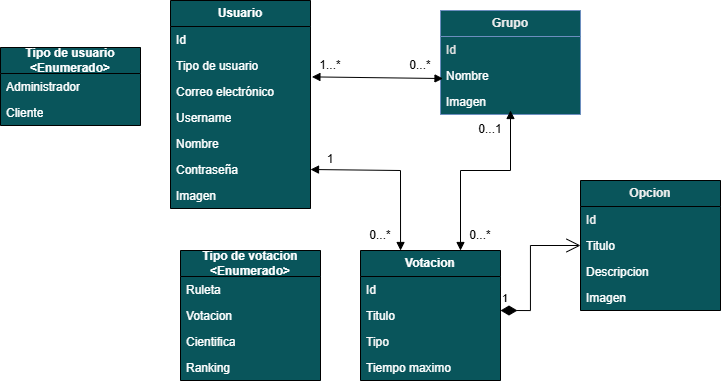
\includegraphics[width=\tamInterfaz\textwidth]{figuras/diagramas/DiagramaClases1.png}
    \caption{Diagrama de clases de análisis }
    \label{fig:diagramaclases1}
\end{figure}